\chapter{3-lagen architectuur: introductie van Spring Data JPA}

De Spring Boot applicaties die we tot nu toe hebben gebouwd bestaand uit 2 lagen. De RestController uit de router-laag gebruikt de functionaliteit of business-logica uit de service-laag.
Nu voegen we een derde laag toe aan de Spring Boot applicaties: de persistence-laag. Deze laag is verantwoordelijk om gegevens op te halen en weg te schrijven naar de databank.

Oze RESTful webapplicaties bestaan dus uit 3 lagen:
routerlaag (of API-laag), service- of bedrijfslogicalaag en persistentielaag.

\begin{itemize}
\item \textbf{Router- of presentatielaag:} Het afhandelen en verwerken van HTTP-verzoeken, het vertalen van JSON-parameters naar objecten, authenticatie van gebruikers en het beschermen van gegevens tegen kwaadwillige gebruikers, ... .
\item \textbf{Servicelaag:} Deze laag bevat de bedrijfslogica, de kernfunctionaliteit van je applicatie. Alle berekeningen, beslissingen, evaluaties, gegevensverwerking, ... worden door deze laag afgehandeld.
\item \textbf{Data- of persistentielaag:} Deze laag is verantwoordelijk voor de interactie met de database. Deze laag slaat de gegevens op en haalt deze op uit de database.
\end{itemize}

Elke laag heeft zijn eigen annotatie voor Spring Beans:

\begin{itemize}
\item @Component: generieke annotatie voor alle componenten beheerd door Spring
\item @RestController: voor de componenten in de router-laag
\item @Service: voor de componenten in de service-laag
\item @Repository: voor de componenten in de persistentielaag
\end{itemize}


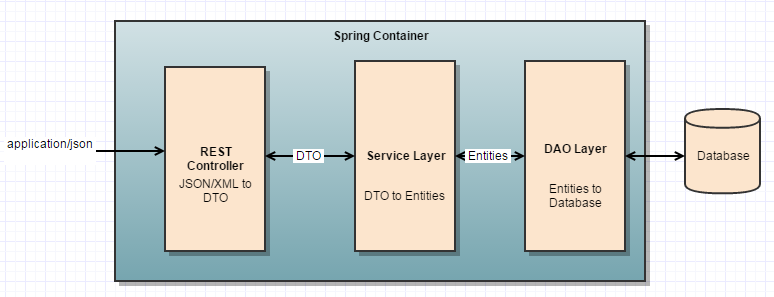
\includegraphics[width=\textwidth]{./images/Spring-REST-Web-Services.png} 

Bovenstaande afbeelding toont alle lagen die we ontwikkelen in een RESTful web applicatie. De RestController in de API-laag biedt REST-endpoints aan. De API-laag communiceert via DTO's of Data Transfer Objects met de servicelaag. De servicelaag implementeert alle bedrijfslogica. DTO's worden omgevormd naar entiteiten.  Entiteiten zijn  objecten uit het domein die we persisteren in de databank.  Deze entiteiten worden  doorgegeven aan de persistentielaag. De persistentielaag is verantwoordelijk voor het opslaan van de entiteiten in de database.

De Spring-container staat centraal in het Spring Framework. De container is verantwoordelijk voor het maken en beheren van objecten voor klassen die zijn geannoteerd met @Service, @Repository, ... De container zal deze objecten (beans) beschikbaar stellen wanneer ze nodig zijn.


\section{Een voorbeeld toepassing}

Dit hoofdstuk begeleidt je bij het ontwikkelen van een Spring Boot-toepassing waarbij we gegevens gaan wegschrijven naar en ophalen uit een databank. Je implementeert een RESTful web applicatie om de gegevens  maken om de informatie van de `Superhero Company' te beheren.  We zullen REST-endpoints implementeren voor het creëren,  aanpassen en verwijderen van superhelden. Later voeg je functionaliteit toe om missies voor de superhelden te creëren,  te updaten en te verwijderen. 

We gebruiken Spring Initializr om deze Spring Boot-toepassing op te zetten.

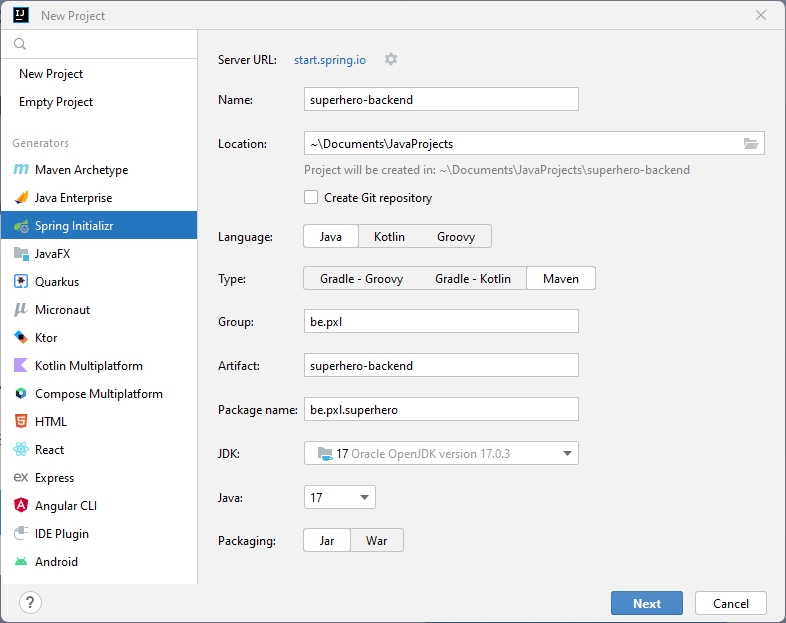
\includegraphics[width=\textwidth]{./images/chapter2/new_project.png} 

Vul de metadata voor het project in. Gebruik Maven als build tool. 


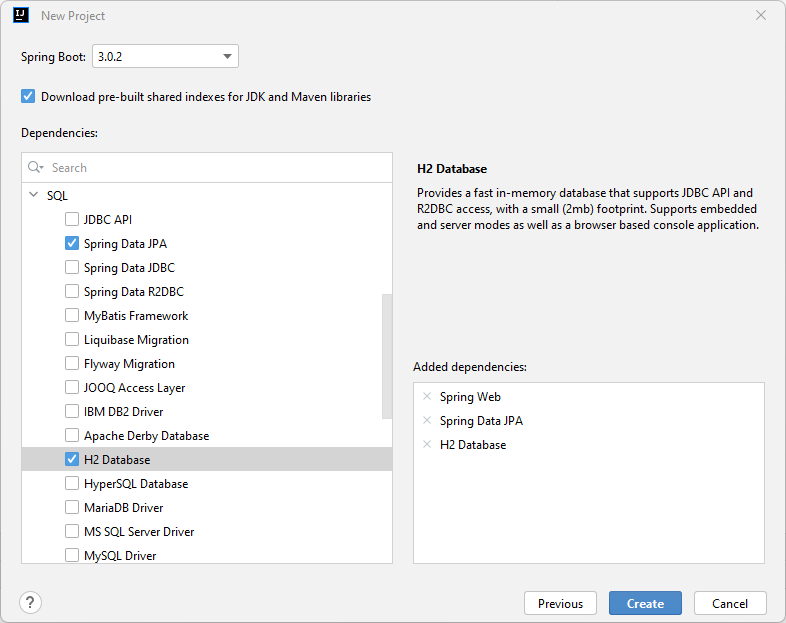
\includegraphics[width=\textwidth]{./images/chapter2/new_project_metadata.png}


\begin{oefening}
Maak het Spring Boot project met de naam `superhero-backend' aan.  Naast Spring Web en Spring Validation voeg je ook Spring Data JPA toe aan het project. Tenslotte voeg je nog de H2 Database dependency toe. Dit is een in-memory database en je hebt amper configuratie nodig om deze database te gebruiken. Dit is handig voor snelle prototyping, maar al je gegevens gaan verloren zodra je de toepassing opnieuw start.
\end{oefening}

\section{Gegevens opslaan en ophalen}

\subsection{Entiteitsklasse Superhero}

Allereerst hebben we een klasse nodig om de objecten te representeren die worden opgeslagen en opgehaald uit de database. Elk object van deze klasse zal overeenkomen met één rij van een tabel in de relationele database.
We implementeren de klasse Superheld. Om Superheld-objecten in de database op te slaan en deze later uit de database op te halen, annoteren we deze klasse als een entiteit. Een entiteitsklasse vertegenwoordigt een entiteit of object in het domeinmodel en wordt gemapt naar een tabel in de database. Elke instantie van deze klasse komt overeen met een rij in deze tabel, waardoor de eigenschappen van het object worden opgeslagen als kolommen in de database.

Hier is de enteitsklasse Superhero:

\begin{lstlisting}[frame=single]
package be.pxl.superhero.domain;

import jakarta.persistence.Entity;
import jakarta.persistence.GeneratedValue;
import jakarta.persistence.GenerationType;
import jakarta.persistence.Id;
import jakarta.persistence.Table;

@Entity
@Table(name="superheroes")
public class Superhero {
	
	@Id
	@GeneratedValue(strategy = GenerationType.IDENTITY)
	private Long id;
	
	private String firstName;
	private String lastName;
	private String superheroName;

	public Superhero() {
		// JPA only
	}

	public Superhero(String firstName, String lastName, String superheroName) {
		this.firstName = firstName;
		this.lastName = lastName;
		this.superheroName = superheroName;
	}

	public Long getId() {
		return id;
	}

	public String getFirstName() {
		return firstName;
	}

	public void setFirstName(String firstName) {
		this.firstName = firstName;
	}

	public String getLastName() {
		return lastName;
	}

	public void setLastName(String lastName) {
		this.lastName = lastName;
	}

	public String getSuperheroName() {
		return superheroName;
	}

	public void setSuperheroName(String superheroName) {
		this.superheroName = superheroName;
	}

	@Override
	public String toString() {
		return superheroName;
	}
}
\end{lstlisting}

De annotatie @Entity geeft aan dat de klasse Superhero een entiteitsklasse is. Spring is in staat om automatisch de databasetabel ('superheroes') te genereren met de nodige kolommen (velden) in de H2-database.
De primaire sleutel van de tabel is gemarkeerd met de annotatie @Id.  Met de annotatie @GeneratedValue(strategy = GenerationType.IDENTITY), hoeven we de primaire sleutels niet toe te wijzen aan de objecten. De database zelf is verantwoordelijk voor het genereren en toewijzen van de primaire sleutels.

\begin{oefening}
Voeg de enteitsklasse Superhero toe aan het project. Je voegt deze klasse toe in het package \textit{be.pxl.superhero.domain}.
\end{oefening}

\subsection{Repository}

Om query's in de database uit te voeren, hebben we een extra interface nodig die een \textbf{repository} wordt genoemd. Spring is in staat om automatisch databasequery's te genereren. Wanneer je de interface JpaRepository uitbreidt, zijn eenvoudige query's (zoals save, findById,...) al beschikbaar zonder dat je een regel code hoeft te schrijven.
De generieke interface JpaRepository hoeft alleen maar te weten welke gegevens het moet opslaan en ophalen.
Daarom moet het de naam van de entiteitsklasse en het gegevenstype van de primaire sleutel van de entiteitsklasse weten.

\begin{lstlisting}[frame=single]
package be.pxl.superhero.repository;

import be.pxl.superhero.domain.Superhero;
import org.springframework.data.jpa.repository.JpaRepository;
import org.springframework.stereotype.Repository;

@Repository
public interface SuperheroRepository extends JpaRepository<Superhero, Long> {
}
\end{lstlisting}



\begin{oefening}
Bestudeer de documentatie van de generieke interface JPARepository.
Voeg de repository SuperheroRepository toe  in het project.  Maak hiervoor het package \textit{be.pxl.superhero.repository} aan.
\end{oefening}

\subsection{Service-layer}

Zoals je al weet is de service-laag verantwoordelijk voor de implementatie van de businesslogica. De klassen in de service-laag zullen gebruik maken van repostories en andere service-klassen.  

Het is een goede idee om voor elke klasse in de servicelaag een interface te voorzien.
De serviceklassen mogen nooit entiteitsobjecten retourneren. We hebben DTO's (Data Transfer Objects) nodig om gegevens van de servicelaag naar de API-laag te sturen.

\begin{lstlisting}[frame=single]
package be.pxl.superhero.service;

import be.pxl.superhero.api.SuperheroDTO;
import be.pxl.superhero.api.SuperheroRequest;

import java.util.List;

public interface SuperheroService {

	List<SuperheroDTO> findAllSuperheroes();

	SuperheroDTO findSuperheroById(Long superheroId);

	Long createSuperhero(SuperheroRequest superheroRequest);

	SuperheroDTO updateSuperhero(Long superheroId, SuperheroRequest superheroRequest);

	boolean deleteSuperhero(Long superheroId);
}
\end{lstlisting}


\begin{lstlisting}[frame=single]
package be.pxl.superhero.api;

import be.pxl.superhero.domain.Superhero;

public class SuperheroDTO {

	private final Long id;
	private final String firstName;
    private final String lastName;
    private final String superheroName;

    public SuperheroDTO(Superhero superhero) {
	   this.id = superhero.getId();
        this.firstName = superhero.getFirstName();
        this.lastName = superhero.getLastName();
        this.superheroName = superhero.getSuperheroName();
    }

	public Long getId() {
		return id;
	}

	public String getFirstName() {
        return firstName;
    }

    public String getLastName() {
        return lastName;
    }

    public String getSuperheroName() {
        return superheroName;
    }

}
\end{lstlisting}

\begin{lstlisting}[frame=single]
package be.pxl.superhero.api;

public class SuperheroRequest {

	private String firstName;
	private String lastName;
	private String superheroName;

	public SuperheroRequest(String firstName, String lastName, String superheroName) {
		this.firstName = firstName;
		this.lastName = lastName;
		this.superheroName = superheroName;
	}

	public String getFirstName() {
		return firstName;
	}

	public void setFirstName(String firstName) {
		this.firstName = firstName;
	}

	public String getLastName() {
		return lastName;
	}

	public void setLastName(String lastName) {
		this.lastName = lastName;
	}

	public String getSuperheroName() {
		return superheroName;
	}

	public void setSuperheroName(String superheroName) {
		this.superheroName = superheroName;
	}

}

\end{lstlisting}

De klasse SuperheroServiceImpl, geannoteerd met @Service, biedt de implementatie voor de interface SuperheroService.
Alle CRUD-operaties (create-read-update-delete) voor Superhero-objecten worden hier aangeboden.
In de klasse SuperheroServiceImpl wordt alle bedrijfslogica geïmplementeerd. Als we bijvoorbeeld moeten controleren of de superheldennaam van een superheld uniek is, is deze klasse de plek om deze controle uit te voeren. 

De SuperheroRepository wordt door Spring Boot ter beschikking gesteld in de SuperheroServiceImpl. Daarom kan de serviceklasse gegevens opslaan en ophalen uit de database met behulp van deze repository.

\begin{lstlisting}[frame=single]
package be.pxl.superhero.service.impl;

import be.pxl.superhero.api.SuperheroDTO;
import be.pxl.superhero.api.SuperheroRequest;
import be.pxl.superhero.domain.Superhero;
import be.pxl.superhero.exception.ResourceNotFoundException;
import be.pxl.superhero.repository.SuperheroRepository;
import be.pxl.superhero.service.SuperheroService;
import org.springframework.stereotype.Service;

import java.util.List;
import java.util.stream.Collectors;

@Service
public class SuperheroServiceImpl implements SuperheroService {

	private final SuperheroRepository superheroRepository;

	@Autowired
	public SuperheroServiceImpl(SuperheroRepository superheroRepository) {
		this.superheroRepository = superheroRepository;
	}

	public List<SuperheroDTO> findAllSuperheroes() {
		return superheroRepository.findAll()
				.stream().map(SuperheroDTO::new)
				.toList();
	}

	public SuperheroDTO findSuperheroById(Long superheroId) {
		return superheroRepository.findById(superheroId)
		         .map(SuperheroDTO::new)
				.orElseThrow(() -> new ResourceNotFoundException("Superhero", "ID", superheroId));
	}

	public Long createSuperhero(SuperheroRequest superheroRequest) {
		Superhero superhero = new Superhero();
		superhero.setFirstName(superheroRequest.getFirstName());
		superhero.setLastName(superheroRequest.getLastName());
		superhero.setSuperheroName(superheroRequest.getSuperheroName());
		Superhero newSuperhero = superheroRepository.save(superhero);
		return newSuperhero.getId();
	}

	public SuperheroDTO updateSuperhero(Long superheroId, SuperheroRequest superheroRequest) {
		return superheroRepository.findById(superheroId).map(superhero -> {
			superhero.setFirstName(superheroRequest.getFirstName());
			superhero.setLastName(superheroRequest.getLastName());
			superhero.setSuperheroName(superheroRequest.getSuperheroName());
			return new SuperheroDTO(superheroRepository.save(superhero));
		}).orElseThrow(() -> new ResourceNotFoundException("Superhero", "id", superheroId));
	}

	public boolean deleteSuperhero(Long superheroId) {
		return superheroRepository.findById(superheroId)
				.map(superhero -> {
					superheroRepository.delete(superhero);
					return true;
				}).orElseThrow(() -> new ResourceNotFoundException("Superhero", "id", superheroId));

	}
}
\end{lstlisting}

\begin{lstlisting}
package be.pxl.superhero.exception;

@ResponseStatus(HttpStatus.NOT_FOUND)
public class ResourceNotFoundException extends RuntimeException {
    public ResourceNotFoundException(String resource, String field, String value) {
        super("Not found: " + resource + " with " + field + "=" + value);
    }

    public ResourceNotFoundException(String resource, String field, long value) {
        this(resource, field, Long.toString(value));
    }
}
\end{lstlisting}

\begin{oefening}
Maak het pakket \textit{be.pxl.superhero.api} aan en voeg het request-object SuperheroRequest en de DTO SuperheroDTO toe. Deze klassen worden gebruikt voor communicatie met de API-laag. Voeg de interface SuperheroService en de implementatie SuperheroServiceImpl toe aan je project. De interface bevindt zich in het pakket \textit{be.pxl.superhero.service}. De implementatie staat in het package \textit{be.pxl.superhero.service.impl}. Voeg tot slot de uitzonderingsklasse ResourceNotFoundException toe aan het package \textit{be.pxl.superhero.exception}.
\end{oefening}

\subsection{RESTController}

Nu kunnen we de REST-endpoints toevoegen voor het creëren, bijwerken, verwijderen en ophalen van superhelden.

Voor het creëren van een nieuwe superheld gebruiken we een POST-verzoek met een requestbody in JSON-formaat. Deze requestbody bevat alle informatie over de nieuwe superheld. Je hebt de klasse SuperheroRequest al aan het project toegevoegd. Deze klasse wordt gebruikt om de gegevens van de requestbody naar een object te mappen.

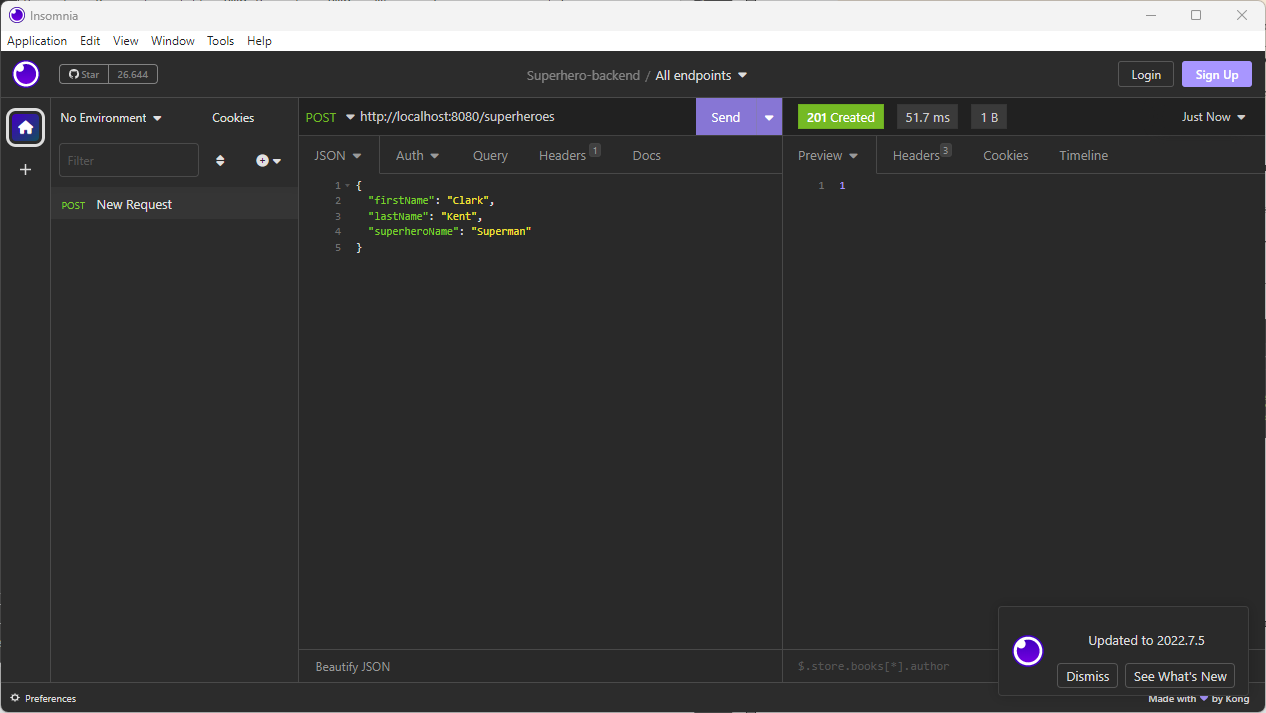
\includegraphics[width=\textwidth]{./images/chapter2/post-request-insomnia.png} 


\begin{lstlisting}[frame=single]
package be.pxl.superhero.api;

import be.pxl.superhero.service.SuperheroService;
import org.springframework.http.HttpStatus;
import org.springframework.http.ResponseEntity;
import org.springframework.web.bind.annotation.DeleteMapping;
import org.springframework.web.bind.annotation.GetMapping;
import org.springframework.web.bind.annotation.PathVariable;
import org.springframework.web.bind.annotation.PostMapping;
import org.springframework.web.bind.annotation.PutMapping;
import org.springframework.web.bind.annotation.RequestBody;
import org.springframework.web.bind.annotation.RequestMapping;
import org.springframework.web.bind.annotation.RestController;

import java.util.List;

@RestController
@RequestMapping("/superheroes")
public class SuperheroController {

	private final SuperheroService superheroService;

	public SuperheroController(SuperheroService superheroService) {
		this.superheroService = superheroService;
	}

	@GetMapping
	public List<SuperheroDTO> getSuperheroes() {
		return superheroService.findAllSuperheroes();
	}

	@GetMapping("/{superheroId}")
	public SuperheroDTO getSuperheroById(@PathVariable Long superheroId) {
		return superheroService.findSuperheroById(superheroId);
	}
	
	@PostMapping
	public ResponseEntity<Long> createSuperhero(@RequestBody SuperheroRequest superheroRequest) {
		return new ResponseEntity<>(superheroService.createSuperhero(superheroRequest), HttpStatus.CREATED);
	}
	
	@PutMapping("/{superheroId}")
	public SuperheroDTO updateSuperhero(@PathVariable Long superheroId, @RequestBody SuperheroRequest superheroRequest) {
		return superheroService.updateSuperhero(superheroId, superheroRequest);
	}
	
	@DeleteMapping("/{superheroId}")
	public ResponseEntity<Void> deleteSuperhero(@PathVariable Long superheroId) {
		boolean deleted = superheroService.deleteSuperhero(superheroId);
		return deleted? new ResponseEntity<>(HttpStatus.OK) : new ResponseEntity<>(HttpStatus.BAD_REQUEST);
	}
}
\end{lstlisting}

\begin{oefening}
Voeg @RestController SuperheroController toe aan je Spring Boot-toepassing. Herstart het project en maak een nieuwe superheld aan met Insomnia of Postman. Vervolgens roep je het REST-eindpunt aan om alle superhelden op te halen of om de superheld op te halen op basis van ID.

Hier is het JSON-formaat om een superheld te creëren:
\begin{lstlisting}
{
	"firstName": "Clark",
	"lastName": "Kent",
	"superheroName": "Superman"
}
\end{lstlisting}
\end{oefening}

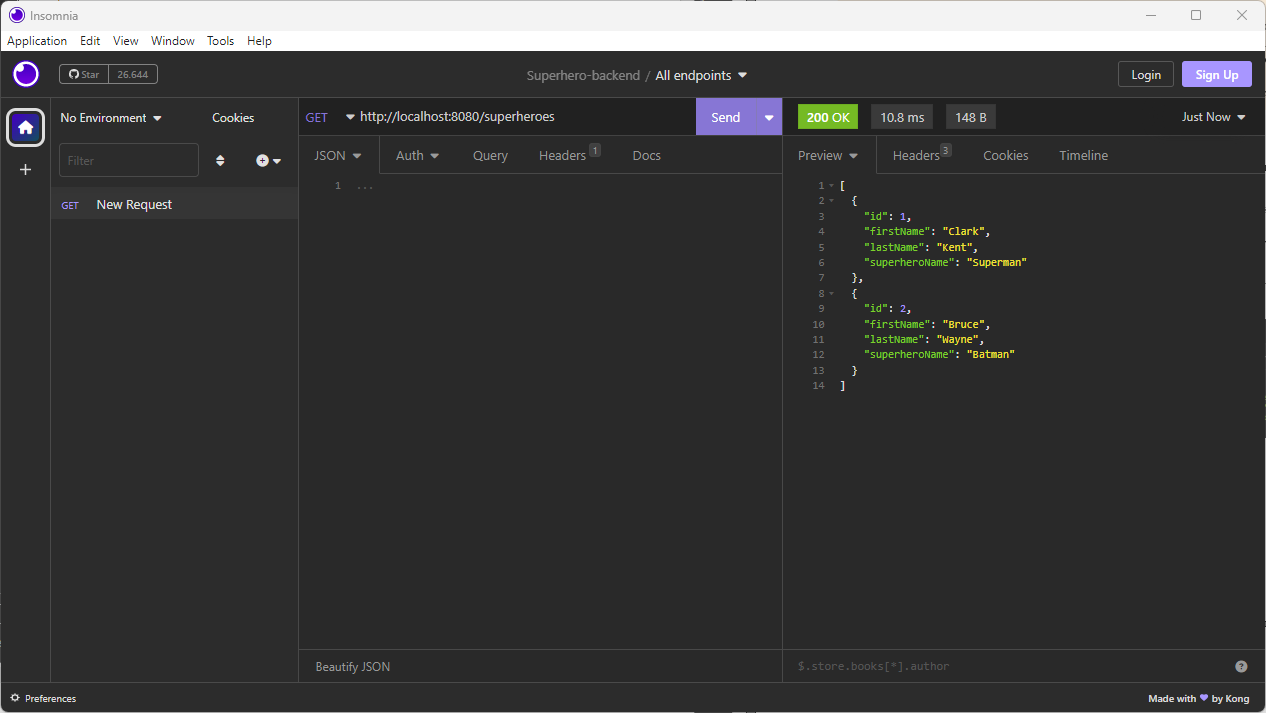
\includegraphics[width=\textwidth]{./images/chapter2/get-request-insomnia.png}

\section{URL context path}

Wanneer je een voorvoegsel (prefix), bijv. /api, aan alle URL's van de applicatie wilt toevoegen, kun je het volgende sleutel-waarde-paar toevoegen in het bestand application.properties:

\begin{lstlisting}[frame=single]
server.servlet.context-path=/api
\end{lstlisting}


\begin{oefening}
Verander het context-pad van je Spring Boot-applicatie. Het voorvoegsel /api moet worden gebruikt voor de applicatie. Herstart de applicatie en test de endpoints.
\end{oefening}

\section{API documentation}



\begin{lstlisting}[language=xml]
<dependency>
			<groupId>org.springdoc</groupId>
			<artifactId>springdoc-openapi-starter-webmvc-ui</artifactId>
			<version>2.2.0</version>
		</dependency>
\end{lstlisting}

De Swagger-documentatie in XML-formaat die te vinden is op de URL \url{http://localhost:8080/api/v3/api-docs} is niet gebruiksvriendelijk. Als je echter de URL \url{http://localhost:8080/api/swagger-ui.html} opent in je browser, kun je een gebruiksvriendelijke Swagger-pagina zien waar je zelfs je API kunt testen.

\begin{oefening}
Voeg swagger documentatie toe aan het project. Zoek eens op hoe je bijkomende Swagger documentatie in je RESTController kan toevoegen.
\end{oefening}


\begin{tcolorbox}[colback=blue!5!white,colframe=blue!75!black,title=H2 database]
De H2 in-memory database verdwijnt wanneer je de applicatie afsluit en alle data gaat verloren.
Je kunt bestanden gebruiken om de data permanent op te slaan. Als je de data van je in-memory database wilt bekijken, kun je de volgende eigenschap toevoegen aan het bestand application.properties:
\begin{lstlisting}[frame=single]
spring.h2.console.enabled=true
\end{lstlisting}
Als je de Spring Boot applicatie opstart, krijg je de unieke naam van de database. 
\begin{lstlisting}[frame=single]
H2 console available at '/h2-console'. Database available at 'jdbc:h2:mem:f5f92e54-3aff-4986-9d00-a0028b0eb6ed'
\end{lstlisting}
Als je de URL \url{http://localhost:8080/api/h2-console} in een browser browser open en de unieke naam van de databank invult en username ``sa'' en blanco paswoord ingeeft, dan krijg je toegang tot de tabellen en gegevens van de in-memory databank. 

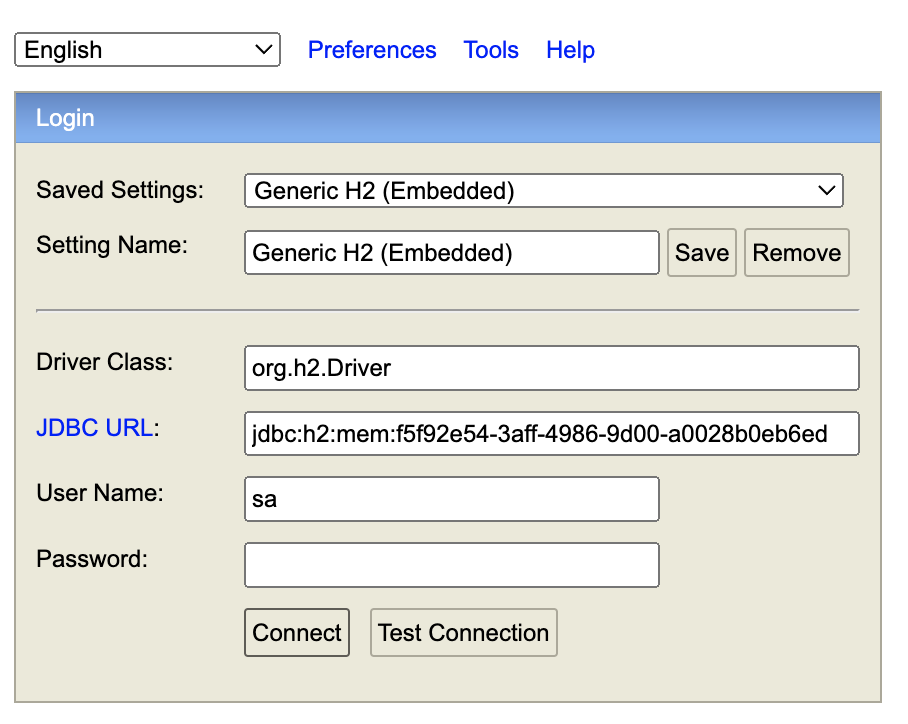
\includegraphics[width=\textwidth]{./images/chapter2/h2-database.png} 

\end{tcolorbox}

\section{Frontend}

Een frontend voor the superhero applicatie, geschreven in Angular,  kan je vinden op github.  (Credits to: \url{https://github.com/shoul10}).


 \fcolorbox{black}[HTML]{ADD8E6}{\parbox{\textwidth}{%
\noindent \textbf{Source code}\\
De frontend code is beschikbaar op: \url{https://github.com/custersnele/superhero-frontend.git}
}}

Zorg ervoor dat de nodige configuratie voorziet zodat de frontend de backend kan bereiken.  Denk eraan dat je ook CORS (Cross-Origin Resource Sharing) moet toestaan in je Spring Boot applicatie.

\begin{oefening}
Voeg CORS-ondersteuning toe aan je project. Voeg de configuratie toe in het package \textit{be.pxl.superhero.config}.  Herstart de Spring Boot applicatie.
Download de frontend code van github en open de code in een ontwikkelomgeving zoals   WebStorm.  Start de frontend toepassing op (ng serve) en cre\"er, update en verwijder je superhelden.
\end{oefening}